\documentclass[10pt]{beamer}
\usetheme{Warsaw}
\usepackage{polski}
\usepackage[utf8]{inputenc}
\title{Continuous Delivery}
\author{Marcin Fabrykowski}
\institute{Alior Bank S.A.}
\begin{document}
\begin{frame}
\titlepage
\end{frame}
\begin{frame}
\frametitle{Kot na dziś}
\begin{center}

\includegraphics[width=25em]{funny-cat-and-computer_1.jpg}
\end{center}
\end{frame}
\begin{frame}
\frametitle{O czym bedzie}
\tableofcontents
\end{frame}
\section{Continuous Delivery}
\begin{frame}[fragile]
\frametitle{Continuous Delivery}
Ciocia Wikipedia:\\
\begin{verbatim}
Continuous delivery (CD) is a software engineering approach
in which teams produce software in short cycles, ensuring
that the software can be reliably released at any time.
It aims at building, testing, and releasing software
faster and more frequently. The approach helps reduce the cost,
time, and risk of delivering changes by allowing
for more incremental updates to applications in production.
A straightforward and repeatable deployment process
is important for continuous delivery.
\end{verbatim}
\pause
bla bla bla...
\end{frame}
\begin{frame}
\frametitle{Continuous Delivery}

\includegraphics[width=30em]{a-komu.png}
\end{frame}
\begin{frame}
\frametitle{A komu to potrzebne?}
\begin{center}
\vskip-0.5cm

\includegraphics[width=0.4\textwidth]{sysadmin.jpg}
\end{center}
\pause
\begin{columns}[t]
\column{.5\textwidth}
\begin{center}
\vskip-1cm

\includegraphics[width=0.2\textwidth]{sad.png}
\end{center}
\begin{itemize}
\item cp
\item unzip
\item stop/start
\item select/update
\end{itemize}
\pause
\column{.5\textwidth}
\begin{center}
\vskip-1cm

\includegraphics[width=0.2\textwidth]{smile.png}
\end{center}
\begin{itemize}
\item strace
\item tuning
\item ansible
\item koty w internecie
\end{itemize}
\end{columns}
\end{frame}
\begin{frame}
\frametitle{Przepływ według Wikipedii}
\begin{center}
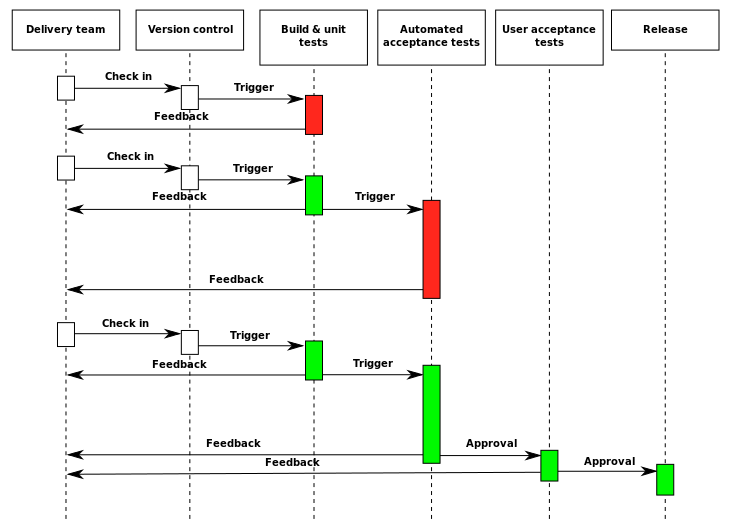
\includegraphics[width=0.9\textwidth]{diagram.png}
\end{center}
\end{frame}
\section{Tools}
\subsection{Rundeck}
\begin{frame}
\frametitle{Rundeck}
\begin{center}

\includegraphics[width=0.7\textwidth]{rundeck.png}
\end{center}
Rundeck is open source software that helps you automate routine operational procedures in data center or cloud environments. Rundeck provides a number of features that will alleviate time-consuming grunt work and make it easy for you to scale up your automation efforts and create self service for others. 
\end{frame}
\subsection{Ansible}
\begin{frame}
\begin{center}

\includegraphics[width=0.3\textwidth]{ansible.png}
\end{center}
Ansible is an open-source automation engine that automates software provisioning, configuration management, and application deployment.
\end{frame}
\subsection{Vagrant}
\begin{frame}
\begin{center}

\includegraphics[width=0.3\textwidth]{vagrant.png}
\end{center}
Vagrant is an open-source software product for building and maintaining portable virtual software development environments
\end{frame}
\subsection{RPM}
\begin{frame}
\begin{center}

\includegraphics[width=0.3\textwidth]{500px-RPM_Logo.png}
\end{center}
RPM Package Manager (RPM) (originally Red Hat Package Manager; now a recursive acronym) is a package management system.
\end{frame}
\section{Stachu, jak się to robi?}
\subsection{Określenie wymagań}
\begin{frame}
\frametitle{Określenie wymagań}
Cele główne:
\begin{enumerate}
\item{Deploy aplikacji}
\item{Minimalizacja czasu deployment-u}
\item{Brak niedostępności}
\end{enumerate}
\end{frame}
\subsection{Krok po kroku}
\begin{frame}
\frametitle{Krok po kroku}
Jak się do tego zabrać:
\begin{enumerate}
\item{postawienie maszyny (opcjonalne)}
\item{przygotowanie systemu}
\item{przygotowanie serwera aplikacyjnego}
\item{wypięcie z balancerów}
\item{deploy aplikacji}
\item{testy}
\item{wpięcie do balancerów}
\end{enumerate}
\end{frame}
\subsection{Best practices}
\begin{frame}
\frametitle{Na co zwrócić uwagę?}
Jak robić, to dobrze...\\
czyli jak?
\begin{enumerate}
\item{idempotencja!!!}
\item{wykorzystanie dostępnych modułów}
\item{prostota}
\item{unikanie 'command' i 'shell'}
\item{tagowanie tasków}
\item{podział inventory na środowiska}
\item{deduplikacja kodu}
\end{enumerate}
\end{frame}
\section{Demo?}
\begin{frame}
\frametitle{Demo?}
Demo?
\end{frame}
\end{document}
